\documentclass{article}
\usepackage[utf8]{inputenc}
\usepackage{graphicx}
\usepackage{hyperref}
%\usepackage[a4paper,width=150mm,top=1in,bottom=1in]{geometry}
%\usepackage[a4paper,margin=1in]{geometry}
\usepackage{indentfirst}

\usepackage{amsmath}
\pagenumbering{arabic}
\usepackage{subcaption}
\usepackage[numbered]{mcode}    %using mcode.sty to convert .m file code to latex format
\usepackage{listings}
\usepackage{adjustbox}
\usepackage{minted}
\graphicspath{{./images/}}

\lstset{
  basicstyle=\ttfamily,
  columns=fullflexible,
  frame=single,
  breaklines=true,
  postbreak=\mbox{\textcolor{red}{$\hookrightarrow$}\space},
}

\begin{document}

\begin{titlepage}
    % --------------------------------------------------------------------
    % Formatting title layout
    % --------------------------------------------------------------------
    \newcommand{\HRule}[1]{\rule{\linewidth}{#1}} 	% Horizontal rule
    \makeatletter							% Title
    \def\printtitle{%						
        {\centering \@title\par}}
    \makeatother									
    
    \makeatletter							% Author
    \def\printauthor{%					
        {\centering \large \@author}}				
    \makeatother							

    % --------------------------------------------------------------------
    % Title text
    % --------------------------------------------------------------------
    \title{	\normalsize \textsc{} 	% Subtitle
    		 	\\[2.0cm]								% 2cm spacing
    			\HRule{0.5pt} \\						% Upper rule
    			\LARGE \textbf{\uppercase{ECE 161B: Lab 0\\ Discrete-Time Domain Signal in MATLAB}}	% Title
    			\HRule{2pt} \\ [0.5cm]		% Lower rule + 0.5cm spacing
    			\normalsize ECE 161B | WINTER 2020\\
    			\today			% Todays date
    		}
    
    \author{
    		Roy Kim\\	
    		A13804992\\
    		Electrical and Computer Engineering\\	
    		UC San Diego\\
    }
    
    % ------------------------------------------------------------------------------
    % Title display (Maketitle)
    % ------------------------------------------------------------------------------
    \thispagestyle{empty}		% Remove page numbering on this page
    
    \printtitle					% Print the title data as defined above
      	\vfill
    \printauthor				% Print the author data as defined above
    \newpage

\end{titlepage}

% ------------------------------------------------------------------------------
% Table of contents
% ------------------------------------------------------------------------------
\hspace{0pt}
\vfill
\tableofcontents
\vfill
\hspace{0pt}
\newpage
% ------------------------------------------------------------------------------
% Content
% ------------------------------------------------------------------------------
\section{Introduction}
    In this lab we will generate a discrete-time domain signal using MATLAB and analyze its power spectrum in the frequency domain. We will learn about \textbf{spectral leakage} and \textbf{signal aliasing}. We will observe aliasing due to under-sampling and how this relates to the Nyquist-Shannon sampling theorem, the minimum required sample frequency to maintain all the signal information is 2 times the frequency of the highest component. We will also write our signal into a ".wav" file, operate on the file, and read the file back into MATLAB.

%    \begin{figure}[h!]
%        \centering
%        \includegraphics[scale=1.7]{universe}
%        \caption{The Universe}
%        \label{fig:universe}
%    \end{figure}

\section{Objectives}
    \begin{enumerate}
      \item Generate a discrete-time domain signal in MATLAB
      \item Write the result to file
      \item Verify the results of your code in MATLAB
    \end{enumerate}

\section{Results}
    \subsection{Task 1.} Sampling sinusoids,
        \begin{align*}
            x_1&=sin(2 \pi f_1 n) & f_1&=2.3kHz\\
            x_2&=sin(2 \pi f_2 n) & f_2&=23kHz\\
            x_3&=sin(2 \pi f_3 n) & f_3&=36kHz
        \end{align*}
        Continuous waveform plot,
        \flushleft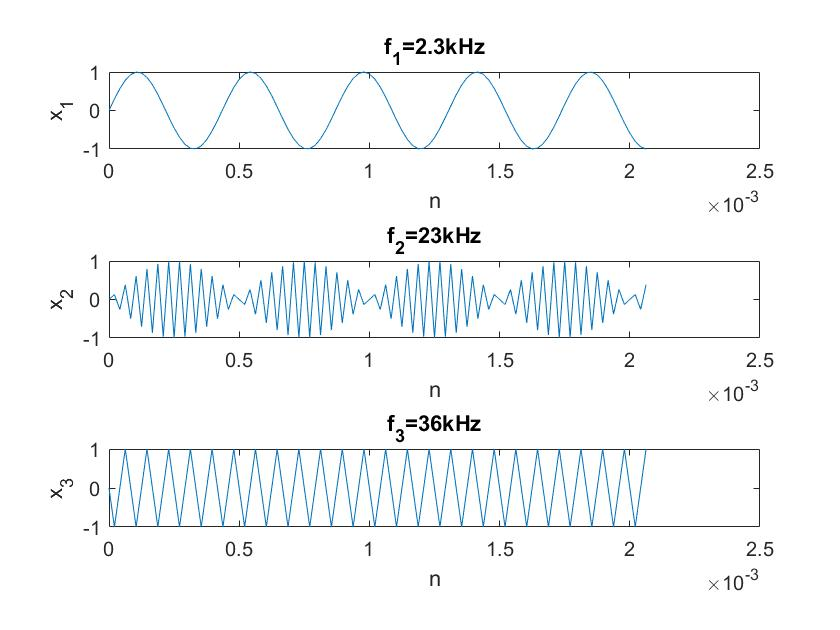
\includegraphics[width=\textwidth]{task1b.jpg}
        Using stem() to get 100-discrete samples, we observe that the waveform looks as below:
        \flushleft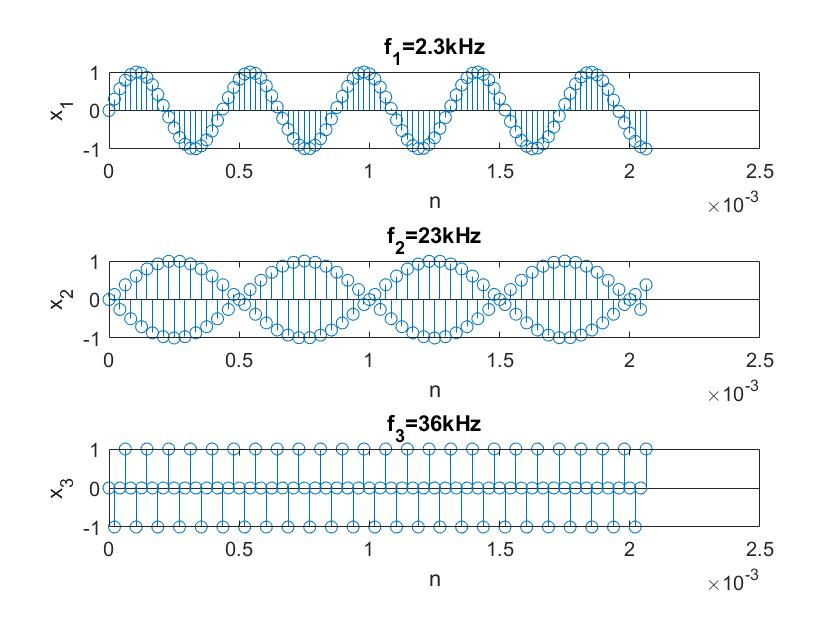
\includegraphics[width=\textwidth]{task1a.jpg}
        Looking at the stem plot, we can easily see the 100 points of each sinusoid--given that $L=100$.\\
        \vspace{5mm}
        From observation the 2.3kHz sinusoid has a longer wavelength than the 36kHz sinusoid, and this we expect because wavelength is inversely proportional to frequency $\lambda=\frac{1}{f}$. So the higher frequency will have a shorter wavelength.\\
        The 23kHz sinusoid looks like an amplituded modulated signal. As if two sinusoids have been added together in such a way that the waveform looks like beats; where there is constructive interference at the peaks and destructive interference at the nodes. Initially, I was expecting to see a sine wave similar to signals $x_1$ and $x_3$ but with a wavelength in between the two.
        
    \subsection{Task 2.}
        \begin{align*}
            X_1&=FFT(x_1) & f_1&=2.3kHz\\
            X_2&=FFT(x_2) & f_2&=23kHz\\
            X_3&=FFT(x_3) & f_3&=36kHz
        \end{align*}
        $X_1$, $X_2$, $X_3$ are power spectrums of their corresponding signals.\\
        \vspace{5mm}
        64-Fast Fourier Transform in radians,
        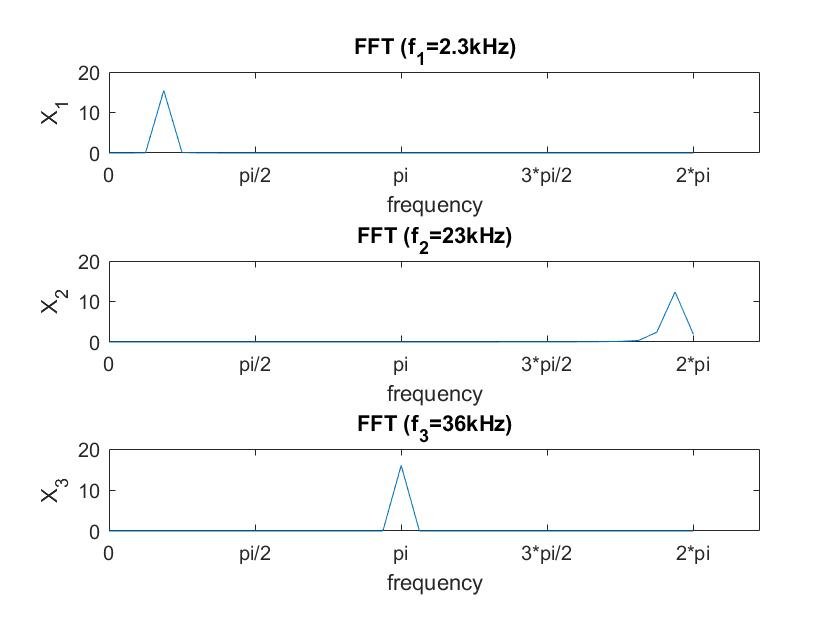
\includegraphics[width=\textwidth]{task2b.jpg}
        \newpage
        For analysis purpose I will observe the power spectral densities in frequency.\\
        FFT in frequency,
        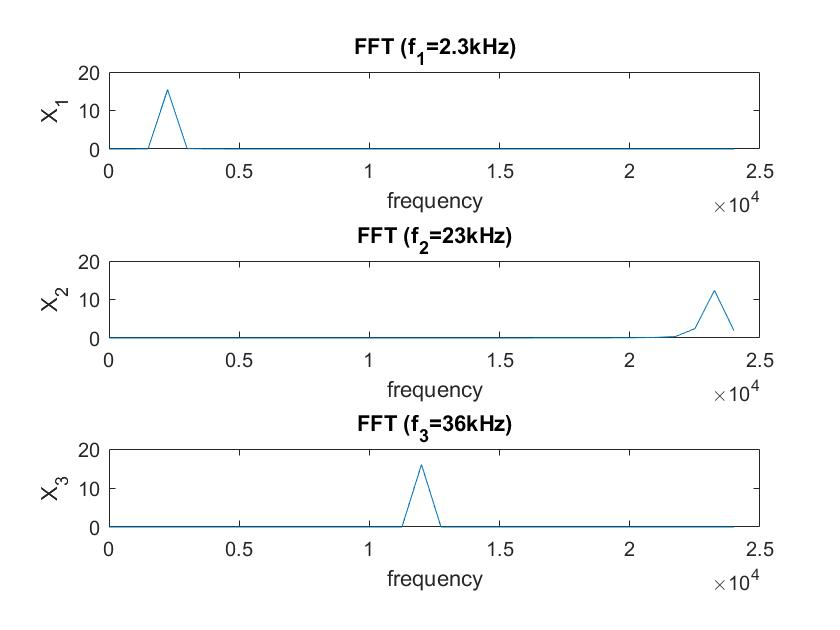
\includegraphics[width=\textwidth]{task2a.jpg}
        From the fft plot in frequency, we can observe that $x_1$ has a frequency of 2.3kHz, $x_2$ has a frequency of 23kHz, and $x_3$ has a frequency that is not 36kHz (between 10kHz and 15kHz); this is due to the under-sampling of signal $x_3$ caused by the sampling rate (discussed in detail in \textbf{Task 4}). However, we do expect to see three distinct peaks in the FFT plot since we have three distinct sinusoids.\\
        \vspace{5mm}
        When taking the fft() of the signals, we plot half the points since we know that sine and cosine have a positive and a negative frequency component in the frequency domain.
        \begin{align*}
            cos(\omega_0 t)=\pi[\delta(\omega-\omega_0)+\delta(\omega+\omega_0)]\\
            sin(\omega_0 t)=\frac{\pi}{2}[\delta(\omega-\omega_0)-\delta(\omega+\omega_0)]
        \end{align*}
        From this Fourier Transform, we expect to see delta functions in the frequency domain analysis. However in our observation, we do not see delta functions. And this is due to \textbf{spectral leakage} (discussed in \textbf{Task 3}) and how MATLAB handles windowing and bins.
        \newpage
        FFT in frequency plotted together,
        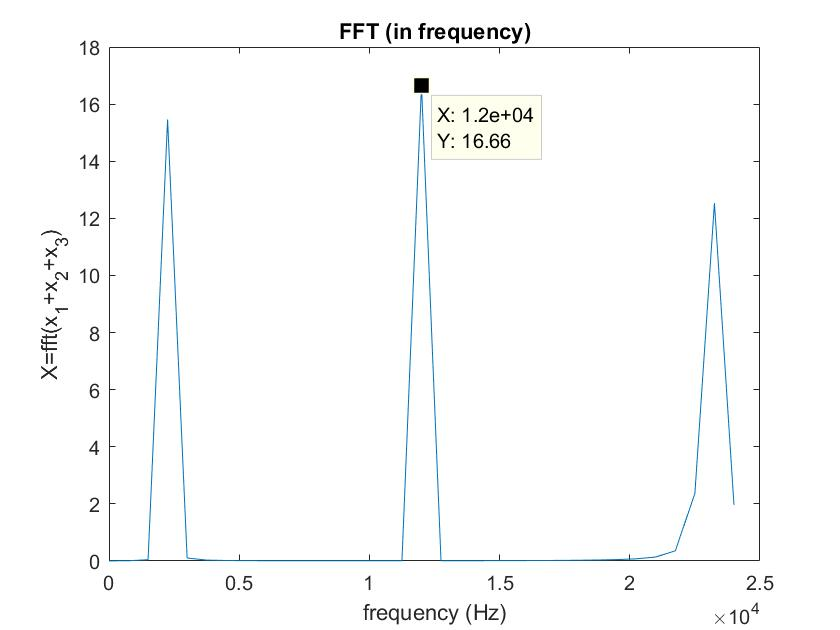
\includegraphics[width=\textwidth]{task2.jpg}
        Here we can better see that signal $x_3$ has been undersampled. It's fft shows that $x_3$ has a frequency component of 1.2kHz when the original signal is 36kHz.
    \subsection{Task 3.} Explain why the magnitude plots are not delta functions.\\
        \vspace{5mm}
        \begin{enumerate}
            \item\url{https://flylib.com/books/en/2.729.1/dft_leakage.html}
            \item\url{https://dspillustrations.com/pages/posts/misc/spectral-leakage-zero-padding-and-frequency-resolution.html}
        \end{enumerate}
        \begin{equation}
            F_{analysis}(k)=k*\frac{f_s}{N}
        \end{equation}
        The magnitude plots of the fft() are not delta functions due to DFT leakage. This is because the "input sequence does not have an integral number of cycles over the N-sampled DFT interval, so the input energy has leaked into all the other DFT output bins."
        \newline
        "the analytical frequencies always have an integral number of cycles over our total sample interval of 64 points."
        \newline
        "the DFT assumes that its input signal is one period of a periodic signal, its output are the discrete frequencies of this periodic signal" (1)\\
        \vspace{5mm}
        Because the DFT assumes a periodic repetition of the signal, we can see from \textbf{Task 1} that our signals are not a complete period with length $L=100$. So there will be discontinuities between the transistions since we did not capture a complete period. So the DFT will not see a pure sinusoidal wave, so we do not see a delta function. This is an example of \textbf{spectral leakage}.\\
        \vspace{5mm}
        "\textbf{spectral leakage} -- even though the signal x(t) is a periodic signal of frequency $f_0$, if we take a part of the signal and calculate the DFT spectrum from it, we see multiple frequencies occuring, due to the strange behaviour at the period's boundary" (2)\\
        \vspace{5mm}
        If we were to measure an integer multiple of the signal period, then we would observe that the leakage would disappear, since the fft() will see a complete periodic signal.
    \pagebreak
    \subsection{Task 4.} Describe how the plots in Task 2 relate to the famous Nyquist-Shannon sampling theorem. (If there is aliasing, at what frequency is it showing it in the spectrum and why?)\\
        \vspace{5mm}
        \begin{center}
            \textbf{\Large{Nyquist-Shannon sampleing theorem:}}\\
            \url{http://195.134.76.37/applets/AppletNyquist/Appl_Nyquist2.html}
            "The minimum sampleing frequency of a signal that it will not distort its underlying information, should be double the frequency of its highest frequency component."
            \newline
            "If $f_s$ is the sampling frequency, then the critical frequency (or Nyquist limit) $f_N$ is defined as equal to $\frac{f_s}{2}$."
        \end{center}
        \vspace{5mm}
        The plots in \textbf{Task 2} show the frequency domain of the signals $x_1$, $x_2$, and $x_3$.
        There is aliasing on signal $x_3$. The original sinusoid has a frequency of 36kHz, but due to aliasing, the 64-fft shows that $x_3$ has a frequency of 12kHz. This means that $x_3$ with a frequency of $f_3=36kHz$ has been \textbf{under-sampled or distorted}, and we can say \textbf{$x_3$ is an aliased signal due to undersampling.}
        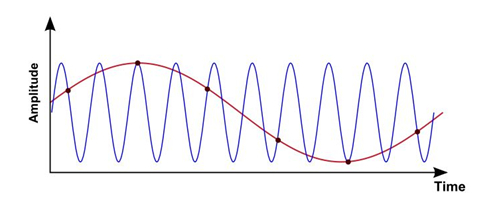
\includegraphics[width=\textwidth]{aliasing.jpg}
        \newline\newline
        This can be explained by the Nyquist-Shannon sampling theorem, that says \textit{"The minumum sampling frequency of a signal that it will not distort its underlying information, should be double the frequency of its highest frequency component."}
        \begin{align*}
            x_1&=sin(2 \pi f_1 n) & f_1&=2.3kHz\\
            x_2&=sin(2 \pi f_2 n) & f_2&=23kHz\\
            x_3&=sin(2 \pi f_3 n) & f_3&=36kHz
        \end{align*}
        $F_s=48kHz$ should be used for frequency components $\leq 24kHz$ signals, so $x_1$ and $x_2$ will retain their signal information; frequency components higher than 24kHz will be aliased--as seen with $x_3$ which has a frequency component of 36kHz.\\
        \vspace{5mm}
        The minimum sampling rate to maintain the original signal of all $x_1$, $x_2$, and $x_3$ is $F_N=2\times max(f_1,f_2,f_3)=2 \times 36000=72kHz$
        
    \subsection{Task 5.}
        Used \textbf{audiowrite()} and to write each signal to a wav file. Using the c-file, I generated a c-skeleton that reduced the amplituded of the signals by one half in an output wav file. I then read the signal back into MATLAB using \textbf{audioread()}.\\
        \vspace{5mm}
        Plotting the processed signals from the c-generated file,
        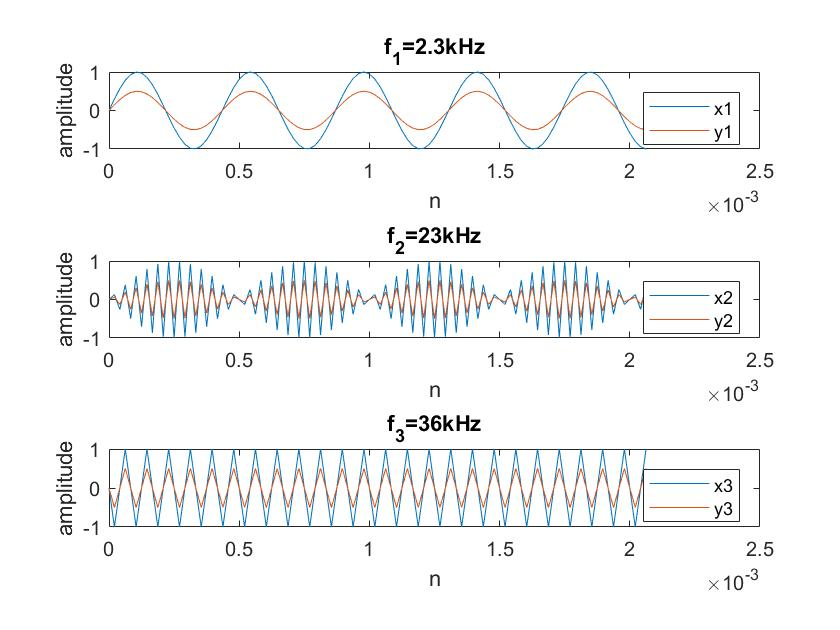
\includegraphics[width=\textwidth]{task5.jpg}
        \begin{center}
            $x$ is the original signal\\
            $y$ is the modified signal
        \end{center}
        The c-generated wav files show an output signal that has a max amplitude of one half. This verifies that the c-skeleton did reduce the amplitudes of each signal by half. Without changing the shape of the waveform, we reduced the amplitudes by dividing by two each component of the signal, element by element wise.
\newpage
\section{Code Appendix}
    \subsection{MATLAB Code:}
        %\begin{adjustbox}{max width=\textwidth}
            \lstinputlisting[frame=single]{code-files/lab0.m} 
        %\end{adjustbox}
    \newpage
    \subsection{C Code:}
        \lstinputlisting[frame=single]{code-files/Lab0.c}
    \newpage
    \subsection{\LaTeX Code:}
        \lstinputlisting[frame=single]{main.tex}
\end{document}
